
\documentclass[12pt]{article}
\usepackage{tikz}
\usepackage{pgfplots}
\usepackage{geometry}
\geometry{
  a4paper,
  total={170mm,257mm},
  left=20mm,
  top=20mm,
}
\usepackage{listings}
\lstset{
  basicstyle=\ttfamily,
  columns=fullflexible,
  frame=single,
  breaklines=true,
  postbreak=\mbox{\textcolor{red}{$\hookrightarrow$}\space},
}
\begin{document}
\author{Andrew Phuoc Nguyen (z5162792)}
\title{COMP3331 Assignment Report}
\maketitle
\section{Report Questions}
\subsection{}
\textit{A brief discussion of how you have implemented the STP protocol. Provide a list of features that you 
have successfully implemented. In case you have not been able to get certain features of STP working, 
you should also mention that in your report. }
\newline 
\newline The STP protocol is implemented in the Sender and Receiver class in the logic of its methods and as the actual packet in the STP class. Supporting class Logger is contained in receiver and sender and its sole purpose is to record the logs and collect data for the final summary. The PLD class affects the transmission of packets to simulate real life transmissions. 
\newline The features that work are:
\begin{itemize}
    \item Basic ACK and SEQ number usage
    \item Send file
    \item Receive file
    \item PLD module
    \item Resend previous ACKs upon unexpected ACKs (not fully working)
    \item Error correction (partial)
    \item Timeout
    \item Fast Retransmit
    \item Setup
    \item Set-up
    \item Teardow
    \item Checksum
    \item Buffer out of order packets (not fully working)
    \item Log (final summary not fully reliable)
\end{itemize}  
Unimplemented features:
\begin{itemize}
    \item Calculating RTT (sample and dev)
\end{itemize}  
\subsection{}
\textit{ A detailed diagram of your STP header and a quick explanation of all fields (similar to the diagrams that we have used in the lectures to understand TCP/UDP headers)}
\newline 
\begin{figure}
  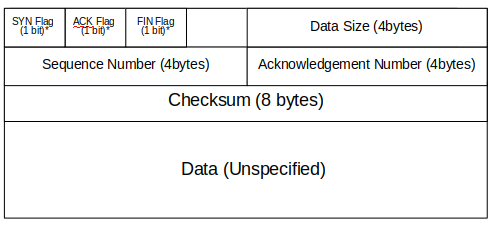
\includegraphics[width=\linewidth]{stp-datagram.png}
  \caption{STP Diagram.}
\end{figure}
\newline * Note that boolean is not defined in Java and thus its size is dependent on the JVM used. All other values are based on Java primitives.
\newline SYN Flag - Notifies receiver that the sender wishes to initiate a file transfer and to form a connection.
\newline ACK Flag - Notifies the receiver that the packet contains no data and signifies an acknowledgement of receiving data.
\newline FIN Flag - Notifies receiver that the sender has completed their operation and that they have completed their portion of the teardown process and they the other may proceed with their teardown. 
\newline Data Size - The number of bytes of data sent in the packet.
\newline Sequence Number - First byte of a segment.
\newline Acknowledgement Number - Notified receiver that the data has been received up to the ACK number.
\newline Checksum - A numerical hash of the rest of the packet using CRC32 used to identify any changes in the packet during transmission.
\newline Data - Data being transmitted.
\subsection{}
\textit{Discuss any design trade-offs considered and made. Describe possible improvements and extensions to your program and indicate how you could realise them.}
\newline
\newline Trade-offs made is in the use of Java as the language to implemenet the protocol as the object-oriented language is relatively slower and inefficient compared to lower level languages such a C. However it made creating STP packets much easier due to classes which allowed for the grouping and scoping of related information. Additionally there is a lot of calculations done on the receiver and sender which could have been offset on the packet to make the server-side calculations shorter such as the relative segment of the packet being sent, mws, mss, and total file size. However this reduces the number of repetitive data being sent. 
\newline Improvements, apart from implementing the incomplete features, include congestion control which would have increased the maximum window size as the packets succeeded in being sent. This increase could have made sending the file a much faster process as fewer segments are needed with larger MWS. This can be achieved on the sender side by collating successful ACKs (matches expected ACK) and unsuccessful ACKs ( those not matching expected ACK) and either doubling, increasing or returning to a MWS of 1, according to the congestion control protocol used. 
\subsection{}
\textit{Indicate any segments of code that you have borrowed from the Web or other books.}
\newline No code from web sources were lifted directly.
\subsection{}
\textit{Questions.}

\end{document}
